\documentclass[12pt,a4paper]{article}
\synctex=1
\usepackage[utf8]{inputenc}
\usepackage[margin=1cm]{geometry}
\usepackage{graphicx}
%\usepackage{verbatim}
\usepackage{amsmath}
\usepackage{amsfonts}
\usepackage{amssymb}
\usepackage{listings}
\usepackage{enumitem}
\usepackage{textcomp}
\usepackage{courier}
\usepackage{libertine}
\usepackage{pgfornament}
\usepackage{eso-pic}
\usepackage[hangul]{kotex}
\linespread{1.3}

\title{
	\centering
	\pgfornament[width=12cm,color=teal]{84}\\
	\vspace{1cm}
	\fontsize{50}{50} \selectfont {정보통신 수학 및 실습\\Homework}\\
		\pgfornament[width=12cm,color=teal]{88}\\
	\vfill}
\author{
	\LARGE
	\begin{tabular}{rl}
		\hline
		학번 : & 2016110056\\ 
		학과 : & 불교학부 \\
		이름 : & 박승원\\
		날짜 : & \today\\
		\hline
	\end{tabular}\vspace{2cm}
	\\
\includegraphics[width=0.5\textwidth]{logo.jpg}
	}
\date{}


\begin{document}
\maketitle
\pagenumbering{gobble}
\noindent
\lstset{language=matlab, columns=flexible, tabsize=4, frame=shadowbox, showstringspaces=false, breaklines=true, upquote=true, basicstyle=\normalsize}

\renewcommand{\thesubsubsection}{\alph{subsubsection})}
\renewcommand{\thesubsection}{\arabic{subsection}.}
\newpage
\section*{Chapter 4 Homework}

\subsection{Find the polar forms of the following complex numbers.}

\subsubsection{$\cos(\dfrac{\pi}{4})+jsin(\dfrac{\pi}{4})$}
$e^{j\frac{\pi}{4}}$
\subsubsection{$\dfrac{1}{\sqrt{2}}+j\dfrac{1}{\sqrt{2}}$} 
$e^{j\frac{\pi}{4}}$
\subsection{Change the following polar forms to complex numbers.} 
\subsubsection{$5\angle\pi$}
$5(\cos\pi + j\sin\pi)=5(-1)=-5$
\subsubsection{$2\angle\dfrac{\pi}{4}$}
$2(\dfrac{1}{\sqrt{2}}+j\dfrac{1}{\sqrt{2}})=\sqrt{2}+j\sqrt{2}$
\subsection{Simplify the following complex numbers.} 
\subsubsection{$\dfrac{2+j5}{3-j}$}
$\dfrac{1}{10} + \dfrac{17 i}{10}$
\subsubsection{$j(5+2j)(3-j)$} 
$-1+17i$
\subsection{Find the phasor whose magnitude is 5 [V], frequency is 60Hz	and initial phase is $\dfrac{\pi}{4}$.} 
$5e^{j2\pi 60 (t+\frac{\pi}{4})}$
\subsection{Find the distance between two complex number z1=x1+jy1 and z2=x2+jy2.}
$\sqrt{(x1-x2)^2+(y1-y2)^2}$
\subsection{Find the coordinates of the following complex numbers and plot them.}
\subsubsection{$-\sqrt{-1}$}
\includegraphics[width=0.8\textwidth]{6a.eps}
\subsubsection{$62\angle 60 + 12\angle 30$}
\begin{lstlisting}
plot(62*e**(i*60)+12*e**(i*30))
\end{lstlisting}

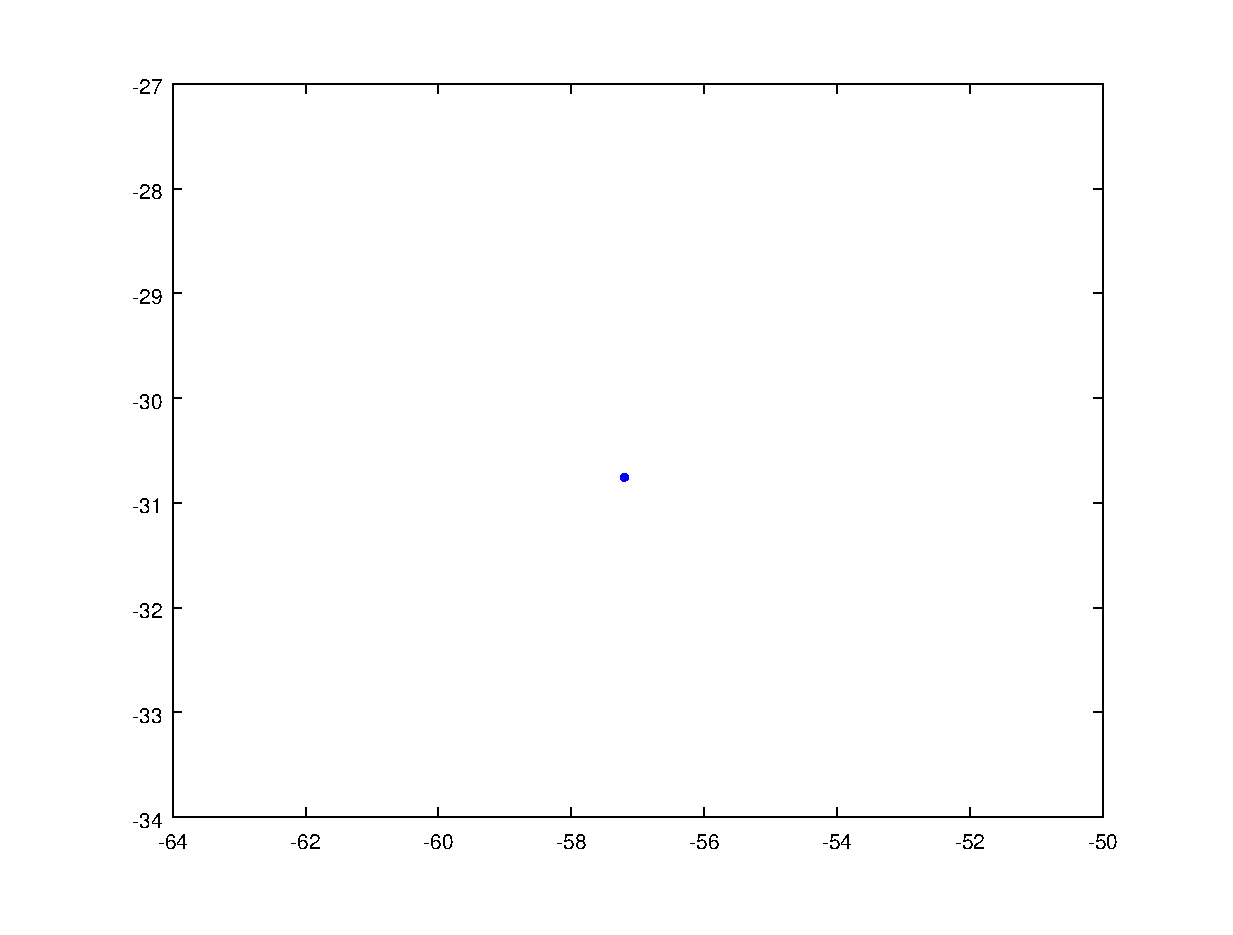
\includegraphics[width=0.8\textwidth]{6b.eps}
\end{document}
